\documentclass[a4paper, 12pt]{article}

%%% Работа с русским языком
\usepackage{cmap}					% поиск в PDF
\usepackage{mathtext} 				% русские буквы в формулах
\usepackage[T2A]{fontenc}			% кодировка
\usepackage[utf8]{inputenc}			% кодировка исходного текста
\usepackage[russian]{babel}	% локализация и переносы

%%% Дополнительная работа с математикой
\usepackage{amsmath,amsfonts,amssymb,amsthm,mathtools} % AMS
\usepackage{icomma} % "Умная" запятая: $0,2$ --- число, $0, 2$ --- перечисление

%% Номера формул
%\mathtoolsset{showonlyrefs=true} % Показывать номера только у тех формул, на которые есть \eqref{} в тексте.

%% Шрифты
\usepackage{euscript}	 % Шрифт Евклид
\usepackage{mathrsfs} % Красивый матшрифт

%% Поля
\usepackage[left=2cm,right=2cm,top=2cm,bottom=2cm,bindingoffset=0cm]{geometry}

%% Русские списки
\usepackage{enumitem}
\makeatletter
\AddEnumerateCounter{\asbuk}{\russian@alph}{щ}
\makeatother

%%% Работа с картинками
\usepackage{graphicx}  % Для вставки рисунков
\graphicspath{{images/}{images2/}}  % папки с картинками
\setlength\fboxsep{3pt} % Отступ рамки \fbox{} от рисунка
\setlength\fboxrule{1pt} % Толщина линий рамки \fbox{}
\usepackage{wrapfig} % Обтекание рисунков и таблиц текстом

%%% Работа с таблицами
\usepackage{array,tabularx,tabulary,booktabs} % Дополнительная работа с таблицами
\usepackage{longtable}  % Длинные таблицы
\usepackage{multirow} % Слияние строк в таблице

%% Красная строка
\setlength{\parindent}{2em}

%% Интервалы
\linespread{1}
\usepackage{multirow}

%% TikZ
\usepackage{tikz}
\usetikzlibrary{graphs,graphs.standard}

%% Верхний колонтитул
\usepackage{fancyhdr}
\pagestyle{fancy}

%% Перенос знаков в формулах (по Львовскому)
\newcommand*{\hm}[1]{#1\nobreak\discretionary{}
	{\hbox{$\mathsurround=0pt #1$}}{}}

%% Мои дополнения
\usepackage{float} %Добавляет возможность работы с командой [H] которая улучшает расположение на странице
\usepackage{gensymb} %Красивые градусы
\usepackage{graphicx}               % Импорт изображений
\usepackage{caption} % Пакет для подписей к рисункам, в частности, для работы caption*

% подключаем hyperref (для ссылок внутри  pdf)
\usepackage[unicode, pdftex]{hyperref}

%%% Теоремы
\theoremstyle{plain}                    % Это стиль по умолчанию, его можно не переопределять.
\renewcommand\qedsymbol{$\blacksquare$} % переопределение символа завершения доказательства

\newtheorem{theorem}{Теорема}[section] % Теорема (счетчик по секиям)
\newtheorem{proposition}{Утверждение}[section] % Утверждение (счетчик по секиям)
\newtheorem{definition}{Определение}[section] % Определение (счетчик по секиям)
\newtheorem{corollary}{Следствие}[theorem] % Следстиве (счетчик по теоремам)
\newtheorem{problem}{Задача}[section] % Задача (счетчик по секиям)
\newtheorem*{remark}{Примечание} % Примечание (можно переопределить, как Замечание)
\newtheorem{lemma}{Лемма}[section] % Лемма (счетчик по секиям)

\begin{document}
    \newcommand{\HRule}{\rule{\linewidth}{0.7mm}} % Defines a new command for the horizontal lines, change thickness here
	
	\begin{center}
		\large\textbf{Московский Физико-Технический Институт}\\ % Name of your university/college
		\large\textbf{(государственный университет)}
	
		\vfill
		
		\Large Лабораторная работа по курсу общей физики № *labnum*\\[0.5cm] % Preambule of your document title
		
		
		\HRule
		\\[0.4cm]
		{ \huge \bfseries *name of your labwork*}% Title of your document
		\\[0.4cm] 
		\HRule
		\\[0.5cm]
		
		\ \\
	\textbf{\large Автор:} \\	
	\large *your name* *groupname*\\ % Your name and something more, your group num for example
		\vfill
		\hspace*{-0.8 cm}
\includegraphics[width=100 pt]{frkt_logo}\\ % logo of your  company/university/college
		\large Долгопрудный, 2021 % location and year
	\end{center}

\newpage
\setcounter{page}{2}
\fancyfoot[c]{\thepage}
\fancyhead[L] {Работа № *labnum*} % some information in page header
\fancyhead[R]{}

    \section*{Цель работы}

    \section*{Теоретическая чать}

    \subsection{Частица над потенциальной ямой}

    Запишем уравнения Шредингера в общем виде

    \begin{equation}
        -\frac{\hbar^2}{2mc} \psi'' + U \psi = E \psi
    \end{equation}

    \[ \psi'' + \frac{2mc}{\hbar^2}(E - U) \psi = 0 \]

    Рассмотрим потенциальную яму глубиной $U_0$ и шириной $l$.

    \begin{figure}
        \centering
        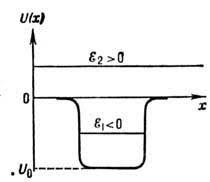
\includegraphics[scale=1]{ph.jpeg}
        \caption{Потенциальная яма}
        \label{fig:ph}
    \end{figure}

    Тогда для области вне ямы уравнение запишется

    \begin{equation}
        \psi'' + \frac{2mc}{\hbar^2} E = 0
    \end{equation}

    где $E$ -- потенциальная энергия частицы. А для области внутри ямы уравнение запишем

    \begin{equation}
        \psi'' + \frac{2mc}{\hbar^2}(E + U_0) = 0
    \end{equation}

    Введем коэффициенты

    \begin{equation}
        k_1^2 = \frac{2mc}{\hbar^2} E
    \end{equation}

    \begin{equation}
        k_2^2 = \frac{2mc}{\hbar^2}(E + U_0)
    \end{equation}

    Приведем качественное объяснение эффекта Рамзауэра.

    Запишем коэффициент прохождения частицы через потенциальную яму

    \begin{equation}
        D = \frac{16 k_1^2 k_2^2}{16 k_1^2 k_2^2 + 4(k_1^2 - k_2^2) \sin^2 (k_2 l)}
    \end{equation}

    Как мы видим, коэффициент прохождения частицы зависит от $\sin^2 (k_2 l)$, а $k_2$ в свою очередь зависит от энергии
    частицы. Именно поэтому при разных энергиях частиц зависимость прохождения частицы над потенциальной ямой разная и имеет
    последовательность минимумов и максимумов. В частности, коэффициент прохождения максимальный, при условии

    \begin{equation}
        k_2 l = \sqrt{\frac{2mc}{\hbar^2}(E + U_0)} l = \pi n ~~ (n = 1, 2, \dots)
    \end{equation}

    Теперь приведем более прикладное объяснение.

    Перейдем от волновых функций частиц к их длинам волн. Частице с энергией $E$ соответсвует длина волны де Бройля

    \begin{equation}
        \lambda = \frac{h}{\sqrt{2mE}}
    \end{equation}

    При прохождении частицы над потенциальной ямой длина волны меняется:

    \begin{equation}
        \lambda' = \frac{h}{\sqrt{2m(E+U_0)}}
    \end{equation}

    Яму в этом случае можно рассматривать в качестве оптически более плотной среды. В таком случае можно рассмотреть
    интерференцию прошедшей и отраженной волн

    \begin{figure}
        \centering
        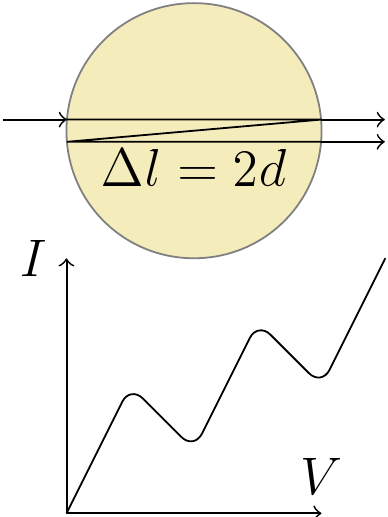
\includegraphics[scale=0.5]{Ramsauer.png}
        \caption{Интерференция волн}
        \label{fig:interf}
    \end{figure}

    Запишем условие на максимум и минимум, $\Delta$ -- оптическая разность хода. Условие на максимум: оптическая разность хода
    равна целому числу полуволн

    \begin{equation}
        \Delta = 2l = 2n \frac{\lambda'}{2} = n \lambda'
    \end{equation}

    Условие на минимум: оптическая разность хода равна полуцелому числу полуволн

    \begin{equation}
        \Delta = 2l = (2n + 1) \lambda'
    \end{equation}

    Таким образом, подставляя в формулы выражения для волны де Бройля, получаем

    \begin{equation}
        \begin{cases}
            2l = \sqrt{\frac{h^2}{2m (E_1 + U_0)}} \\
            2l = \frac{3}{2} \sqrt{\frac{h^2}{2m (E_2 + U_0)}} \\
        \end{cases}
    \end{equation}

    где $E_1$ -- энергия частиц, дающая максимум, $E_2$ -- энергия частиц, дающая минимум, $U_0$ -- глубина потенциальной ямы.

    Решая совместно эти 2 уравнения можно исключить $U_0$ и найти ширину ямы

    \begin{equation} \label{eq:width}
        l = \sqrt{\frac{5 h^2}{32 m (E_2 - E_1)}}
    \end{equation}

    а так же расчитать глубину ямы

    \begin{equation} \label{eq:U_0}
        U_0 = \frac{4}{5}E_2 - \frac{9}{5}E_1
    \end{equation}

    В нашем эксперементе кинетическую энергию частица получает, при прохождении ускоряющей разности потенциалов $E = e V$, 
    где $V$ -- ускоряющая разность потенциалов. Поэтому

    \[ E_1 = e V_1 ~~~ E_2 = e V_2 \]

    \section*{Эксперементальная установка}

    \section*{Обработка эксперементальных данных}
    % m = 9.1 * 10^{-31} кг
    % 1 эВ = 1.6 * 10^{-19} дж
    % h = 2pi * 6.58 * 10^{-16} эВ*с

    % l1 = 3.49 A
    % l2 = 3.19 A
\end{document}